\section{Eswatini HIV Epidemic}\label{intro.esw}
Eswatini\footnote{Officially \emph{the Kingdom of Eswatini},
  and formerly known as \emph{Swaziland} until 2018.}
is a small landlocked country bordering South Africa and Mozambique,
with approximately 1.2 million total population (630,000 aged 15--49) as of 2021 \cite{DataBank}.
Since approximately 2004, Eswatini has had
the highest HIV prevalence in the world (among ages 15--49),
estimated to be 28\% in 2021 \cite{DataBank,AIDSinfo}.
Even within this context, burden of HIV among FSW remains even higher,
estimated around 60\% in 2011 and 2021 \cite{Baral2014,EswIBBS2022}.
Yet, Eswatini was also recently among the first countries in SSA
to achieve the UNAIDS 95-95-95 ART cascade goals \cite{959595,AIDSinfo}.
Thus, Eswatini represents a unique context in which to explore
various modelling assumptions about:
relative drivers of transmission in a high-prevalence epidemic --- including unmet needs of FSW ---
and the potential prevention impacts of ART --- including rapid, yet evidently achievable, scale-up.
This section provides general and HIV-specific context about HIV,
including a summary of the major data sources.
%===================================================================================================
\subsection{Politics \& Society}\label{intro.esw.soc}
Eswatini is divided into four regions: Hhohho, Lubombo, Manzini, and Shiselweni,
each comprising several tinkhundla (administrative subdivisions),
which in turn comprise several imiphakatsi (chiefdoms).
The country gained independence from British colonial rule in 1968,
and remains the last absolute monarchy in Africa
under King Mswati III (1986--present), son of King Sobhuza II (1921--1982) \cite{Mthembu2022}.
Political parties have been officially banned since 1973,
and the monarchy retains powers to
dissolve parliament, veto bills, and appoint most politicians \cite{Maphalala2021}.
Lavish expenditures by the royal family have been criticized \cite{Debly2014,Mthembu2022},
and some authors have argued that cultural traditions and institutions
have been appropriated to entrench and legitimize royal power \cite{Debly2014,Golomski2019}.
Socioeconomic inequality remains high \cite{Debly2014,Kali2023,DataBank},
although economic growth and human development indicators
were above the SSA average prior to the HIV epidemic \cite{Whiteside2007}.
While freedoms of expression remain severely restricted \cite{Debly2014,Mthembu2022},
trade unions act as proxies for political parties,
and calls for democratic reform have recently grown
\cite{Debly2014,Maphalala2021,Mthembu2022,Maseko2023}.
\par
Patriarchal norms are strong in Eswatini and domestic violence is common
\cite{Whiteside2003,Buseh2010,Simelane2011,Dlamini-Simelane2017,Golomski2019}.
Husbands often earn and control most/all household income, and women have reported prioritizing
\shortquote{honour in marriage and performance of being a good wife}~\cite{Dlamini-Simelane2017}.
Married women must usually consult with a ``therapy management group'',
comprising her husband and kin from both sides of the family, before seeking healthcare;
the group may in fact make decisions fully on her behalf \cite{Dlamini-Simelane2017}.
Such barriers can cause substantial delays in accessing HIV treatment \cite{Dlamini-Simelane2017}.
Gender-based food and/or economic insecurity is also a major driver of
transactional sex and sex work within SSA \cite{Scorgie2012}.
\par
Key populations are criminalized in Eswatini, including anybody
buying or selling sex, engaging in same-sex sex acts, or possessing drugs \cite{UNAIDS2022lpa}.
As noted in \sref{intro.hiv.epi.kp}, such laws have substantial implications for
the ability of population-level data and services to reach key populations \cite{WHO2016kp}.
Despite the recognized importance of meeting these populations' prevention needs \cite{EswBSS2002},
specific services were not prioritized for this purpose until approximately 2009 \cite{NERCHA2009}.
%===================================================================================================
\subsection{Eswatini HIV Epidemic \& Response}\label{intro.esw.hiv}
\begin{figure}
  \centering
  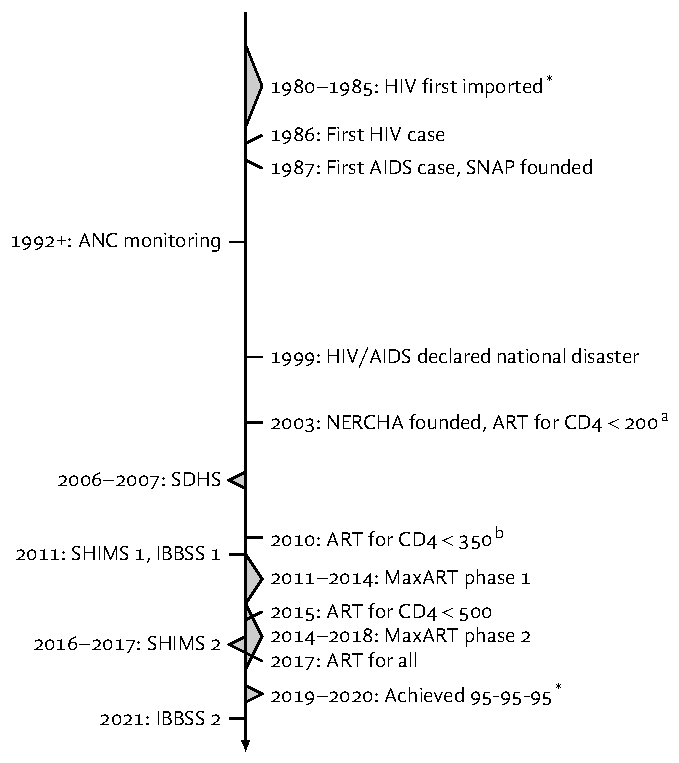
\includegraphics[scale=1]{esw.timeline}
  \caption{Timeline of HIV response in Eswatini}
  \label{fig:esw.timeline}
  \floatfoot{
    \tnt[*]{approximate dates};
    \tnt[a]{plus CD4\,$<$\,350 and WHO stage III, or any CD4 and WHO stage IV};
    \tnt[a]{plus any CD4 and WHO stage III or IV};
    SNAP: Swaziland National AIDS Programme;
    ANC: antenatal care;
    NERCHA: National Emergency Response Council for HIV and AIDS;
    ART: antiretroviral therapy;
    SDHS: Swaziland Demographic and Health Survey;
    SHIMS: Swaziland HIV Incidence Measurement Survey;
    IBBSS: Integrated Biological-Behavioral Surveillance Survey for key populations;
    see also \cite[Figure~3]{Deeks2015} for a timeline of global HIV response.}
\end{figure}
Figure~\ref{fig:esw.timeline} gives a timeline of major events in the Eswatini epidemic response.
The exact timing of HIV introduction to specific countries across SSA, including Eswatini,
remains unclear \cite{Iliffe2005}.
The first cases of HIV and AIDS in Eswatini
were diagnosed in 1986 and 1987, respectively \cite{Whiteside2007}.
Shortly thereafter, the Swaziland National AIDS Programme (SNAP) was founded
within the Ministry of Health as an anchor for the national response \cite{Mabuza2017}.
Yet, with limited tools for treatment and prevention,
HIV prevalence rose rapidly, from 4\% in 1992 to 42\% in 2004
among women attending antenatal care (ANC) clinics
(Figure~\ref{fig:fit.prevalence.anc}) \cite{NERCHA2012}.%
\footnote{ANC data generally overestimate overall HIV prevalence
  due to non-representative sampling \cite{Gouws2008,Marsh2014}.}
Over the same period, crude death rate roughly doubled, magnified by
fragile healthcare infrastructure and a co-epidemic of tuberculosis \cite{Whiteside2007}.
In 2006, 23\% of children under 18 were orphaned (one or both parents were dead),
increasing to 37\% of children aged 15--17,
though not necessarily due to HIV \cite{SDHS2006}.
A more detailed description of HIV incidence and prevalence trends
is given in \sref{model.cal.targ}.
\par
In 1999, King Mswati III declared HIV as a national disaster and
launched the Crisis Management and Technical Committee
to coordinate a multi-sectoral response to the epidemic \cite{Mabuza2017}.
This committe was replaced in 2003 by
the National Emergency Response Council on HIV and AIDS (NERCHA) \cite{Mabuza2017},
which continues to coordinate response via National Strategic Frameworks
over successive 5-year time horizons \cite{NERCHA2009,NERCHA2014,NERCHA2018}.
Also in 2003, ART first became available in Eswatini \cite{NERCHA2012},
after which eligibility and coverage have steadily increased alongside WHO recommendations.
\par
The earliest efforts to prevent sexual HIV transmission in Eswatini focused on
voluntary counselling and testing (VCT), condom promotion, and behaviour change communication,
including specific efforts to reach youth \cite{NERCHA2007}.
While condom use has increased (see also \sref{model.par.beta.condom}),
it's not clear whether numbers of sexual partners have changed over time \cite{Cockcroft2010}.
In 2011, Eswatini began two major HIV campaigns:
\emph{Soka Uncobe}: ``conquer through circumcision'' \cite{SHIMS1} and
\emph{MaxART}: Maximizing ART for Better Health and Zero New HIV Infections \cite{MaxART1,MaxART2}.
\emph{Soka Uncobe} sought to increase male circumcision from 8 to 80\%,
and was bookended by the two Swaziland HIV Incidence Measurement Surveys (\emph{SHIMS})
in 2011 \cite{SHIMS1} and 2016--17 \cite{SHIMS2}.
Despite prior evidence of acceptability and large demand creation efforts,
male circumcision only reached 30\% by 2016 \cite{SHIMS2} and 37\% by 2020 \cite{EswCOP21}.
\emph{MaxART} included two phases with the following specific goals.
Phase~1 (2011--15) sought to:
scale up HIV testing to reach 250,000 people per year,
reach 90\% of eligible PLHIV with ART, and
reduce 1-year ART loss to follow-up from 22\% to 10\%.
Phase~2 (2014--17) sought to:
determine the impact of early ART for all on retention and viral suppression,
assess the role of community engagement in ART scale-up, and
explore differences in systems and experiences pre \vs post intervention.
Most \emph{MaxART} goals were met \cite{MaxART2,Walsh2020},
and Eswatini became one of the first countries globally to
achieve the UNAIDS 95-95-95 goals by 2020 \cite{959595,AIDSinfo}.
Additional details of ART scale-up in Eswatini are given in \sref{model.par.cascade.tx}.
\par
As of the 2018 National Strategic Framework \cite{NERCHA2018},
Eswatini has moved to decentralize the HIV response
and support a broad set of tools to ``micro-target'' local drivers of transmission.
These tools include:
continued promotion of HIV education and condoms,
continued resources for testing and treatment,
structural interventions to reduce gender based violence and stigma \cite{Saul2018},
STI treatment and VMMC services, and
scale-up of PrEP for young women, serodiscordant couples, and key populations.
% TODO: (?) KP-specific interventions
%---------------------------------------------------------------------------------------------------
\subsubsection{Data Sources}\label{intro.esw.hiv.data}
Major HIV data sources for Eswatini are summarized in Table~\ref{tab:esw.data},
and briefly described as follows.
Summary statistics were extracted from reports and publications in all cases,
except two FSW surveys \cite{Baral2014,EswKP2014},
for which individual-level data were obtained and analyzed directly.
\begin{table}
  \centering
  \caption{Main HIV data sources for Eswatini}
  \label{tab:esw.data}
  \begin{tabular}{llllrl}
  \toprule
  Ref & ID & Dates\tn{a} & Population\tn{b} & N\tn{c} & HIV\tn{d} \\
  \midrule
  \cite{SDHS2006}    & DHS'06 & 07/06\,--\,02/07 & GP 15+    &  9,143 & P    \\
  \cite{SHIMS1}      & SHIMS1 & 12/10\,--\,06/11 & GP 18--49 & 18,169 & P, I \\
  \cite{SHIMS2}      & SHIMS2 & 08/16\,--\,03/17 & GP 15+    &  9,146 & P, I \\
  \cite{Baral2014}   & KP'11  & 09/11\,--\,10/11 & KP 15+    &    328 & P    \\
  \cite{EswKP2014}   & KP'14  & 09/14\,--\,01/15 & KP 18+    &    781 & ---  \\
  \cite{EswIBBS2022} & KP'21  & 10/20\,--\,01/21 & KP 18+    &    676 & P, I \\
  \bottomrule
\end{tabular}
\floatfoot{
  \tnt[a]{Baseline data collection (\textsc{mm/yy})};
  \tnt[b]{GP: general population; KP: key populations,
    specifically female sex workers, and men who have sex with men};
  \tnt[c]{Respondents aged xx--49 who completed baseline survey};
  \tnt[d]{Estimates of HIV via blood test, P:~prevalence, I:~incidence}.
}
\end{table}
%---------------------------------------------------------------------------------------------------
\paragraph{General Population}
The 2006--07 Demographic and Health Surey (DHS) \cite{SDHS2006} was
the first nationally representative, household-based survey in Eswatini
covering numerous demographic and health topics.
The survey included dried blood spot HIV testing, covering 88.1\% of women and 81.1\% of men.
Adjusted HIV prevalence was stratified by sex, age, and other demographic factors, as well as
marital status and numbers of sexual partners in the past 12 months (p12m).
The survey also included data on sexual health and behaviour, including
condom use at last sex, STI symptoms in p12m, and HIV testing history.
The two SHIMS in 2010--11 \cite{SHIMS1} and 2016--17 \cite{SHIMS2} were conducted
with the aim of estimating population-level incidence before and after \emph{Soka Uncobe}.
Similar to the DHS, both SHIMS were nationally representative, household-based surveys;
however, SHIMS focused specifically on HIV variables, and additionally estimated
ART cascade steps and HIV incidence.
In SHIMS1 \cite{SHIMS1}, a large prospective 6-month cohort was used to estimate incidence
and validate recency testing \cite{Duong2012} as a cross-sectional measure of incidence, whereas
in SHIMS2 \cite{SHIMS2}, incidence was estimated via the validated recency test.
Compared to the DHS, participation rates were
lower in SHIMS1 (81.7\% and 65.0\% among women and men, for the baseline survey),
and similar in SHIMS2 (88.0\% and 78.5\%).
%---------------------------------------------------------------------------------------------------
\paragraph{Female Sex Workers}
The first behavioural surveillance survey among FSW in Eswatini
reached only 37 FSW during 2001--02 and did not include HIV testing \cite{EswIBBS2022}.
In 2011, a larger survey reached 328 FSW via respondent-driven sampling
and included HIV testing and detailed behavioural data \cite{Yam2013,Baral2014}.
This study found unadjusted HIV prevalence of 70.3\%,
highlighting a concentrated sub-epidemic among this key population
even within the high-prevalence Eswatini epidemic \cite{Baral2014}.
A follow-up study in 2014 aimed to
estimate FSW and MSM population sizes,
identify venues for HIV service delivery, and
provide additional data on service gaps \cite{EswKP2014};
this study used location-based snowball sampling \cite{Weir2005} to reach 781 FSW,
but did not include HIV testing.
Finally, a fourth survey in 2020--21 sought to estimate
FSW and MSM population sizes, HIV prevalence and incidence, prevalence of viral suppression,
as well as identify behavioural and structural factors associated with HIV \cite{EswIBBS2022};
the study recruited 676 FSW via respondent-driven sampling.
